\documentclass[11pt]{article}

% APEL-R: research-level report / paper draft.
% Compile (example): latexmk -pdf apelr.tex

\usepackage[margin=1in]{geometry}
\usepackage{microtype}
\usepackage{amsmath,amssymb,amsthm}
\usepackage{mathtools}
\usepackage{booktabs}
\usepackage{array}
\usepackage{multirow}
\usepackage{graphicx}
\usepackage{hyperref}
\usepackage[capitalize,noabbrev]{cleveref}
\usepackage[numbers,sort&compress]{natbib}
\usepackage{algorithm}
\usepackage{algpseudocode}
\usepackage{tikz}
\usetikzlibrary{positioning,arrows.meta,calc,fit}

\hypersetup{
  colorlinks=true,
  linkcolor=blue,
  citecolor=blue,
  urlcolor=blue,
}

\newcommand{\APEL}{\textsc{APEL}}
\newcommand{\APELR}{\textsc{APEL-R}}

\newcommand{\bvec}{b}
\newcommand{\B}{\mathbf{b}}
\newcommand{\R}{\mathbb{R}}
\newcommand{\V}{\mathcal{V}}
\newcommand{\E}{\mathbb{E}}
\newcommand{\KL}{\mathrm{KL}}
\newcommand{\JS}{\mathrm{JS}}
\newcommand{\softmax}{\mathrm{softmax}}
\newcommand{\Cat}{\mathrm{Cat}}

\newtheorem{theorem}{Theorem}
\newtheorem{proposition}{Proposition}
\newtheorem{definition}{Definition}

\title{\APELR: Asynchronous Planner--Executor Language Modeling\\
with Online Latent-State Filtering and Lookahead Feedback}
\author{Mihir Srivastava\\
\texttt{mihir2k5@gmail.com}}
\date{February 14, 2026}

\begin{document}
\maketitle

\begin{abstract}
We study a model architecture aimed at a specific behavioral objective:
an autoregressive language model that can \emph{plan while speaking}, where the concurrent planning computation can influence the next-token distribution without violating causality.
We present \APEL{} (\textbf{A}synchronous \textbf{P}lanner--\textbf{E}xecutor \textbf{L}anguage modeling), a chunk-latent formulation that separates a fast token-level executor from a slow chunk-level planner.
We then document \APELR{}, a runnable PyTorch prototype that instantiates this idea as a \emph{state-space policy language model}:
it maintains an internal discrete planner belief state updated online by a filtering-style recursion from the realized tokens,
and uses that state to gate a set of expert token heads.
To support ``think-while-speak'' in wall-clock time, the planner can asynchronously forecast future planner beliefs (a lookahead prior) in a background thread and optionally feed the forecast back into the emission gate.

This report is implementation-faithful: we derive the exact and approximate inference modes implied by the factorization, identify a core train--inference mismatch that arises from stale chunk beliefs, and show how \APELR{} tightens the recursion so training and generation share the same causal update semantics.
We present preliminary experiments on TinyStories and WikiText-2 that quantify planner utilization via intervention-style diagnostics (planner masking and forced-state divergences), and ablations demonstrating that (i) online token filtering reduces loss compared to stale chunk beliefs and (ii) lookahead-to-emission feedback can measurably change likelihood under the trained policy.
\end{abstract}

\section{Introduction}
Modern next-token language models exhibit emergent planning-like behaviors, but typical decoding procedures do not allocate explicit compute to planning \emph{concurrently} with token emission.
When ``thinking'' is made explicit (e.g., via chain-of-thought), it is usually produced as additional tokens, entangling internal deliberation with user-visible output.
This motivates architectures that separate an internal planning stream from the emitted token stream:
the model should speak sequentially, while maintaining and updating a compact internal plan state that can be forecast forward and can influence token selection.

This report focuses on a concrete architectural and mathematical question:
\emph{What probabilistic structure admits concurrent planning during autoregressive generation, and what implementation choices are required to keep training and inference aligned?}
We use \APEL{} as the conceptual model class and \APELR{} as the implemented prototype in this repository (\texttt{src/apelr}).

\paragraph{Contributions.}
\begin{enumerate}
  \item We formalize \APEL{} as a chunk-latent autoregressive model and distinguish exact and approximate decoding modes, clarifying where ``exactness'' claims hold (\Cref{sec:apel-model,sec:inference-modes}).
  \item We describe \APELR{} as a \emph{state-space policy LM} in which an internal discrete belief state is updated causally from realized tokens and chunk summaries and gates expert emission heads (\Cref{sec:apelr-arch}).
  \item We specify an asynchronous inference schedule for lookahead forecasting and show what is non-interfering (provably distribution-preserving) versus what is a deliberate policy modification (feedback-coupled lookahead) (\Cref{sec:async}).
  \item We document the objective used in \APELR{}, including auxiliary losses designed to prevent planner bypass and encourage expert specialization (\Cref{sec:training}).
  \item We present preliminary empirical results and ablations on TinyStories and WikiText-2, including intervention-based planner diagnostics and controlled toggles for token filtering and lookahead feedback (\Cref{sec:experiments}).
\end{enumerate}

\begin{figure}[t]
\centering
\resizebox{0.92\linewidth}{!}{%
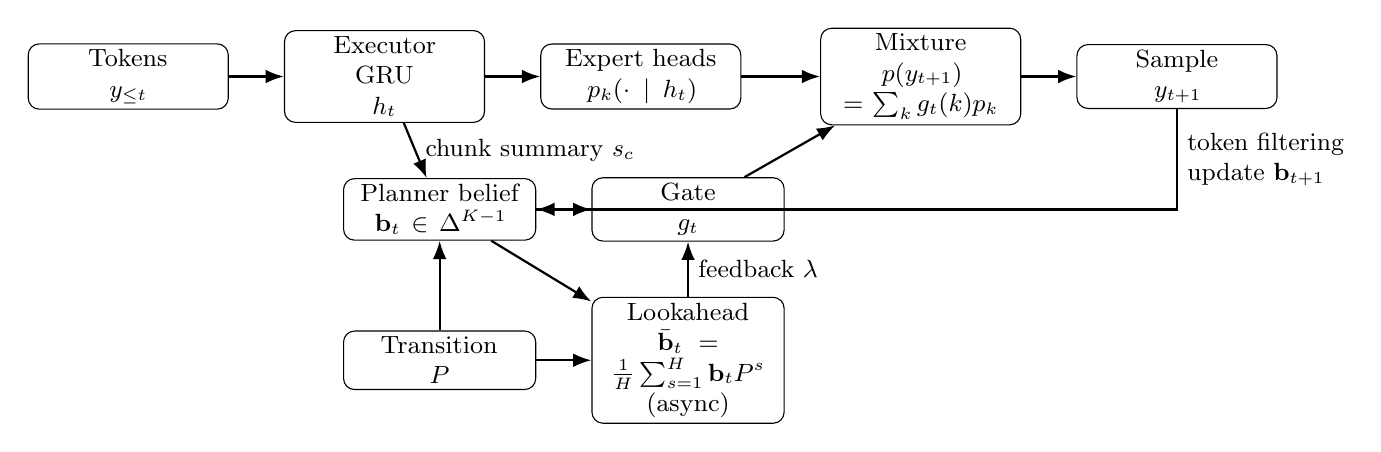
\begin{tikzpicture}[
  node distance=7mm,
  box/.style={draw, rounded corners, align=center, text width=24mm, minimum height=7mm, inner sep=2pt},
  smallbox/.style={draw, rounded corners, align=center, text width=23mm, minimum height=6mm, inner sep=2pt},
  arrow/.style={-Latex, thick},
  every node/.style={font=\small},
]
  \node[box] (tokens) {Tokens\\$y_{\le t}$};
  \node[box, right=of tokens] (gru) {Executor\\GRU\\$h_t$};
  \node[box, right=of gru] (experts) {Expert heads\\$p_k(\cdot\mid h_t)$};

  \node[smallbox, below=of gru, xshift=7mm] (belief) {Planner belief\\$\B_t\in\Delta^{K-1}$};
  \node[smallbox, right=of belief] (gate) {Gate\\$g_t$};

  \node[smallbox, below=of gate] (lookahead) {Lookahead\\$\bar{\B}_t=\frac{1}{H}\sum_{s=1}^H \B_tP^s$\\(async)};
  \node[smallbox, left=of lookahead] (transition) {Transition\\$P$};

  \node[box, right=of experts, xshift=3mm] (mix) {Mixture\\$p(y_{t+1})$\\$=\sum_k g_t(k)p_k$};
  \node[box, right=of mix] (sample) {Sample\\$y_{t+1}$};

  \draw[arrow] (tokens) -- (gru);
  \draw[arrow] (gru) -- (experts);
  \draw[arrow] (experts) -- (mix);
  \draw[arrow] (gate) -- (mix);
  \draw[arrow] (mix) -- (sample);

  \draw[arrow] (sample) |- node[pos=0.25, right, align=left, font=\small] {token filtering\\update $\B_{t+1}$} (belief);
  \draw[arrow] (gru) -- node[midway, right, font=\small] {chunk summary $s_c$} (belief);
  \draw[arrow] (belief) -- (gate);
  \draw[arrow] (transition) -- (belief);
  \draw[arrow] (transition) -- (lookahead);
  \draw[arrow] (belief) -- (lookahead);
  \draw[arrow] (lookahead) -- node[midway, right, font=\small] {feedback $\lambda$} (gate);
\end{tikzpicture}%
}
\caption{Schematic of \APELR{} V2. The executor produces hidden states; experts produce state-conditional token distributions; the planner maintains an online belief over discrete plan states; optional lookahead forecasting can be computed asynchronously and fed back into the gating distribution.}
\label{fig:apelr-v2-schematic}
\end{figure}

\section{Background and Motivation}
\label{sec:background}
\subsection{Why chunk-level planning?}
If a latent plan variable were updated at every token, planning would be entangled with token emission at the same time scale; this can be expressive but offers limited opportunity for parallel planning compute.
Chunking introduces a slow time scale: a plan variable $z_c$ governs a block of tokens.
The planner can then forecast future plan beliefs at chunk granularity (e.g., by applying a transition operator) while the executor emits within a chunk.
This is analogous to hierarchical sequence models and HMM/SSM-style filtering \citep{rabiner1989hmm}.

\subsection{Why a \emph{policy} view?}
In \APELR{}, the planner is not presented as a recovered ground-truth posterior over an external latent variable.
Instead, it is treated as an internal causal state used to parameterize the next-token distribution---i.e., a \emph{policy} for token emission.
The planner state is updated from observed tokens by a filtering-like recursion (a deterministic map into the simplex).
This view is crucial when additional heuristics (e.g., lookahead feedback) are introduced: the resulting model is still a valid conditional distribution over tokens, even if it is not the exact marginal of a particular latent-variable generative story.

\section{\APEL: Chunk-Latent Model Class}
\label{sec:apel-model}
\subsection{Notation}
Let $x$ denote a prompt/context, and $y_{1:T}=(y_1,\dots,y_T)$ denote output tokens with $y_t\in\V$.
Fix a chunk size $m\in\mathbb{N}$ and define chunk index
\[
c(t) := \left\lfloor\frac{t-1}{m}\right\rfloor,\qquad C := \left\lceil \frac{T}{m}\right\rceil.
\]
Chunk $c$ covers token indices $\mathcal{I}_c := \{cm+1,\dots,\min((c+1)m,T)\}$ and begins at $\tau_c := cm+1$.

\subsection{Generative factorization}
\label{sec:factorization}
Introduce a chunk-level latent plan variable $z_c$ (discrete or continuous).
The \APEL{} factorization is:
\begin{equation}
\label{eq:apel-joint}
p_\theta(y_{1:T}, z_{0:C-1}\mid x)
= p_\theta(z_0\mid x)
\prod_{c=0}^{C-2} p_\theta(z_{c+1}\mid z_c, x)\;
\prod_{c=0}^{C-1}\prod_{t\in\mathcal{I}_c} p_\theta(y_t\mid y_{<t}, z_c, x).
\end{equation}
This is a hierarchical latent language model with an autoregressive emission model inside each chunk.

\subsection{Filtering recursion}
Define the chunk-start belief:
\[
\bvec_c(z) := p_\theta(z_c=z\mid x, y_{<\tau_c}).
\]
Within a chunk, the token-time posterior is
\[
\bvec_{c,t}(z) := p_\theta(z_c=z\mid x, y_{<t}),\qquad t\in\mathcal{I}_c.
\]
Let $\ell_t(z) := p_\theta(y_t\mid x, y_{<t}, z_c=z)$.
Then the exact in-chunk Bayes update is:
\begin{equation}
\label{eq:token-filter}
\bvec_{c,t+1}(z)
= \frac{\bvec_{c,t}(z)\,\ell_t(z)}{\sum_{\bar z}\bvec_{c,t}(\bar z)\,\ell_t(\bar z)}.
\end{equation}
At chunk boundaries, define the transition operator $(\mathcal{T}\bvec)(z') := \sum_z p_\theta(z'\mid z,x)\bvec(z)$ (replace the sum by an integral for continuous $z$).
After consuming chunk $c$, the next chunk-start belief is:
\begin{equation}
\label{eq:chunk-boundary}
\bvec_{c+1} = \mathcal{T}\,\bvec_{c,\tau_{c+1}}.
\end{equation}

\subsection{Lookahead as a prior forecast}
At the start of a chunk (or any time at which a belief $\bvec$ is defined), multi-step predictions are:
\begin{equation}
\label{eq:lookahead}
\bvec^{-}_{c+k} = \mathcal{T}^k \bvec_c,\qquad k\ge 1.
\end{equation}
These are priors conditioned only on $(x, y_{<\tau_c})$.
They can be computed without seeing future tokens and thus are compatible with concurrent computation.

\section{Inference Modes and Exactness}
\label{sec:inference-modes}
The factorization in \Cref{eq:apel-joint} admits multiple decoding/inference schedules.
The crucial distinction is whether the belief used to mix emissions is updated token-by-token (exact filtering) or held fixed across a chunk (stale mixture).

\paragraph{Mode A: Ancestral latent sampling (exact).}
At chunk start, sample $z_c\sim \bvec_c$ and then sample each token $y_t\sim p_\theta(y_t\mid y_{<t}, z_c, x)$.
This is exact sampling from the joint and hence yields correct marginals.

\paragraph{Mode B: Token-time filtered mixture (exact for discrete tractable sums).}
At each token position $t\in\mathcal{I}_c$, use
\[
p_\theta(y_t\mid x, y_{<t}) = \sum_z \bvec_{c,t}(z)\, p_\theta(y_t\mid x,y_{<t},z),
\]
and update $\bvec_{c,t+1}$ using \Cref{eq:token-filter}.
This is exact when the sum/integral over $z$ is tractable.

\paragraph{Mode C: Stale chunk mixture (approximate in general).}
Using a fixed chunk-start belief $\bvec_c$ for all $t\in \mathcal{I}_c$,
\[
\tilde p(y_t\mid x, y_{<t}) = \sum_z \bvec_c(z)\, p_\theta(y_t\mid x,y_{<t},z),
\]
is generally approximate unless $\bvec_{c,t}\approx \bvec_c$ throughout the chunk.

\begin{proposition}[Stale chunk mixture is not exact in general]
\label{prop:stale-not-exact}
For the model class in \Cref{eq:apel-joint}, the stale-belief mixture in Mode C equals the true conditional $p_\theta(y_t\mid x,y_{<t})$ for all $t\in \mathcal{I}_c$ only if $\bvec_{c,t}=\bvec_c$ (almost surely) for those $t$.
\end{proposition}
\begin{proof}[Sketch]
The exact conditional requires integrating over $z_c$ with weights $\bvec_{c,t}(z)=p(z_c=z\mid x,y_{<t})$.
When $\ell_t(z)$ depends on $z$, Bayes rule \Cref{eq:token-filter} updates the weights after observing tokens, yielding $\bvec_{c,t}\ne \bvec_c$ except in degenerate cases (e.g., $\ell_t$ independent of $z$ or tokens carry no information about $z$).
\end{proof}

\section{Theoretical Properties for Concurrent Lookahead}
\label{sec:theory}
This section states what can be claimed rigorously about ``planning in parallel'' under the \APEL{} factorization.

\begin{theorem}[Chunk-boundary predict--update identities]
\label{thm:filtering}
Under the factorization in \Cref{eq:apel-joint}, the in-chunk Bayes update \Cref{eq:token-filter} and the chunk-boundary prediction \Cref{eq:chunk-boundary} are exact identities.
\end{theorem}
\begin{proof}[Sketch]
\Cref{eq:token-filter} is Bayes' rule applied to the latent $z_c$ with likelihood $\ell_t(z)$.
\Cref{eq:chunk-boundary} follows from marginalizing $z_c$ and the Markov property of the chunk-level transition $p(z_{c+1}\mid z_c,x)$.
\end{proof}

\begin{theorem}[Asynchronous non-interference for prior lookahead]
\label{thm:noninterference}
Fix a chunk index $c$ and assume decoding uses either Mode A (ancestral latent sampling) or Mode B (token-time filtered mixture) from \Cref{sec:inference-modes}.
Let the planner concurrently compute priors $\bvec_{c+k}^-=\mathcal{T}^k\bvec_c$ during emission of chunk $c$.
If these priors are \emph{not} used to modify the executor's conditional distributions for tokens in chunk $c$, then computing them concurrently does not change the distribution of generated tokens.
\end{theorem}
\begin{proof}[Sketch]
At chunk start, $\bvec_c$ is $\sigma(x,y_{<\tau_c})$-measurable.
The lookahead $\mathcal{T}^k\bvec_c$ is a deterministic function of $(\bvec_c,\theta)$ and hence also $\sigma(x,y_{<\tau_c})$-measurable.
Therefore it is conditionally independent of within-chunk token randomness given the chunk-start information, and computing it in parallel cannot change the conditional used to sample tokens unless it is explicitly fed back to alter those conditionals.
\end{proof}

\begin{theorem}[Parallelizability of discrete lookahead]
\label{thm:parallel}
For discrete $K$-state planner transitions with matrix $P$ and belief vector $\bvec$,
$\bvec P^k$ can be computed with $O(\log k)$ sequential depth via repeated squaring (at the cost of additional parallel matrix multiplications).
\end{theorem}
\begin{proof}[Sketch]
Compute $P^{2^j}$ by squaring: $P^{2^{j+1}}=(P^{2^j})^2$ for $j=0,\dots,\lfloor\log_2 k\rfloor$.
Then express $k$ in binary and multiply the selected powers.
\end{proof}

\section{\APELR: Implementation as a State-Space Policy LM}
\label{sec:apelr-arch}
We now describe the repository implementation, emphasizing what is mathematically exact versus a deliberate engineering choice.

\subsection{High-level architecture}
\APELR{} consists of:
\begin{itemize}
  \item \textbf{Executor (speaker):} a GRU backbone \citep{cho2014gru} that maps the token prefix to a hidden state $h_t\in\R^H$.
  \item \textbf{Planner (thinker):} a discrete belief state $\B_t\in\Delta^{K-1}$ over $K$ planner states, updated causally from realized tokens and chunk summaries.
  \item \textbf{Emission heads:} $K$ expert distributions $p_k(\cdot\mid h_t)$ combined by a gate $g_t\in\Delta^{K-1}$ derived from the planner belief (and optionally its lookahead).
\end{itemize}
The core design goal is bidirectional coupling:
planner state influences token probabilities, and realized tokens update the planner state online (token filtering).

\subsection{Model versions in this repository (V1 and V2)}
\label{sec:model-versions}
This repository implements two versioned architectures (\texttt{docs/model\_versions.md}):
\begin{itemize}
  \item \textbf{V1 (\texttt{v1\_filtered\_mixture}).}
  A filtered-mixture architecture in which a shared emission head is conditioned on a learned plan embedding and a per-plan vocabulary bias (\texttt{src/apelr/model.py}).
  The planner can be under-utilized because experts share substantial capacity.
  \item \textbf{V2 (\texttt{v2\_planner\_required}).}
  A planner-required architecture where token logits are produced by planner-conditioned expert heads only (\texttt{src/apelr/model\_v2.py}).
  V2 also adds explicit planner diagnostics, forced-state interventions, and optional lookahead-to-emission feedback.
\end{itemize}
Both versions maintain an internal discrete belief state and can update it online from realized tokens (token filtering).
V2 primarily tightens identifiability and train--inference alignment by removing a high-capacity bypass path and enforcing a causal chunk-boundary update shared by training and generation.

\subsection{Planner state: discrete latent belief}
In \APELR{} V2, the planner state is a discrete distribution over \emph{latent} states (not literal tokens).
We denote the planner belief before emitting token $t{+}1$ by $\B_t\in\Delta^{K-1}$.
In code, this is a length-$K$ tensor normalized by $\softmax$ (\texttt{model\_v2.py}).

\subsection{Planner transition parameterization}
\label{sec:planner-transition}
\APELR{} implements a simple discrete state-space dynamic:
an initial logit vector $\pi\in\R^K$ and transition logits $A\in\R^{K\times K}$ define
\[
\B_0 = \softmax(\pi),\qquad P_{i,:} = \softmax(A_{i,:}).
\]
The transition matrix $P$ is row-stochastic by construction.
To encourage temporal persistence early in training, $A$ is initialized with a diagonal self-bias:
$A_{ii}\leftarrow \beta$ (config \texttt{planner\_self\_bias}) and $A_{ij}\leftarrow 0$ for $i\ne j$.
This yields a high-probability ``stay'' transition at initialization while preserving learnability.

\begin{definition}[State-space policy language model]
\label{def:ssplm}
A \emph{state-space policy LM} is a model that maintains an internal causal state $s_t$ and defines:
(i) an update rule $s_{t+1}=f_\theta(s_t, o_{t+1})$ driven by observations $o_{t+1}$ available at time $t{+}1$ (e.g., the realized token),
and (ii) an emission policy $\pi_\theta(\cdot\mid s_t, h_t)$ that defines a next-token distribution.
Training typically minimizes next-token cross-entropy under teacher forcing, without requiring $s_t$ to be the posterior of a separate generative latent variable.
\end{definition}

\subsection{Executor and experts}
Given the previous token $y_t$, the GRU updates:
\[
h_t = \mathrm{GRU}(h_{t-1}, e(y_t)),
\]
where $e(\cdot)$ is an embedding.
Each expert $k\in\{1,\dots,K\}$ defines logits $a_{t,k}\in\R^{|\V|}$ and
\[
p_k(y\mid h_t) = \softmax(a_{t,k})_y.
\]
\paragraph{V1 emission parameterization.}
In \APELR{} V1 (\texttt{src/apelr/model.py}), ``experts'' share most parameters and differ through a plan embedding and an explicit per-plan vocabulary bias:
let $u_k\in\R^{d}$ be a learned plan embedding, and let $s_t=W_s h_t + b_s$.
Then a plan-conditioned fusion feature is
\[
j_{t,k}=\tanh(s_t + W_p u_k),
\]
and the per-plan token logits are
\[
a_{t,k} = W_o\, j_{t,k} + b_o + v_k,
\]
where $v_k\in\R^{|\V|}$ is a learned vocabulary-bias vector for plan $k$.
This realizes a filtered mixture-of-experts view \citep{shazeer2017moe}, but because parameters are heavily shared, the model can still reduce planner importance by collapsing plan embeddings/biases.

\paragraph{V2 emission parameterization (planner-required).}
In \APELR{} V2 (\texttt{src/apelr/model\_v2.py}), each plan state has its own linear head,
$a_{t,k}=W_k h_t + b_k$.
This removes a high-capacity shared bypass path and empirically increases intervention sensitivity (forced-state divergences) at comparable training budgets.

\subsection{Token-time filtering update (online coupling)}
\label{sec:token-filtering}
When \texttt{token\_filtering=true}, the belief is updated after observing (or emitting) $y_{t+1}$ using the experts' log-likelihoods:
\begin{equation}
\label{eq:apelr-token-update}
\B_{t+1}
= \softmax\!\left( \log(\B_t+\varepsilon) + \log p_{1:K}(y_{t+1}\mid h_t)\right),
\end{equation}
where $\log p_{1:K}(y\mid h_t)$ denotes the vector of expert log-probabilities for token $y$.
This is the discrete filtering recursion \Cref{eq:token-filter} when the model is interpreted as a discrete latent mixture with tractable emissions; in \APELR{} we adopt it as a causal internal state update (state-space policy).

\subsection{Chunk-boundary update (causal boundary evidence)}
\label{sec:boundary-update}
\APELR{} uses chunking with chunk size $m$.
Let $s_c$ denote a summary of the completed chunk $c$; in the implementation, $s_c$ is the mean of GRU hidden states within the chunk.
At the boundary after completing chunk $c$, the belief is updated by a transition and a boundary-conditioned logit bias:
\begin{equation}
\label{eq:apelr-boundary-update}
\B \leftarrow
\softmax\!\left(
  \log((\B P)+\varepsilon) + \alpha\,W_{\mathrm{bnd}} s_c + W_{\mathrm{obs}} s_c
\right),
\end{equation}
where $P\in\R^{K\times K}$ is a row-stochastic transition matrix and $\alpha$ is a context scale.
This update is \emph{causal}: it depends only on information from the completed chunk.
Importantly, training and generation both apply the same boundary update semantics in V2.

\paragraph{Why ``previous chunk'' evidence matters.}
A common pitfall in hierarchical latent LMs is using information from the \emph{current} chunk to update the chunk's plan state during training, while generation only has partial information mid-chunk.
This creates a train--inference mismatch: the model learns to rely on evidence that does not exist at inference time.
\APELR{} V2 avoids this by defining the boundary update strictly as a function of the \emph{previous} completed chunk summary.
The corresponding implementation is factored into a single helper used by both training and generation (\texttt{\_apply\_boundary\_update}).

\subsection{Emission gate with lookahead feedback}
\label{sec:gate}
Given a current belief $\B_t$ and transition matrix $P$, the planner can forecast future beliefs:
\[
\B_t^{(s)} := \B_t P^s,\qquad s=1,\dots,H.
\]
Define the mean forecast $\bar{\B}_t := \frac{1}{H}\sum_{s=1}^{H}\B_t^{(s)}$.
\APELR{} V2 defines a mixed belief used for gating:
\[
\tilde{\B}_t := (1-\lambda)\B_t + \lambda \bar{\B}_t,\qquad \lambda\in[0,1],
\]
and a temperature-shaped gate:
\begin{equation}
\label{eq:gate-softmax}
g_t := \softmax\!\left(\frac{\log(\tilde{\B}_t+\varepsilon)}{\tau}\right).
\end{equation}
The next-token distribution is then:
\begin{equation}
\label{eq:mixture}
p(y_{t+1}\mid x, y_{\le t})
= \sum_{k=1}^{K} g_t(k)\, p_k(y_{t+1}\mid h_t).
\end{equation}
\paragraph{Interpretation.}
When $\lambda=0$, gating depends only on the current belief (no lookahead feedback).
When $\lambda>0$, the emission distribution is influenced by a concurrent prior forecast of future planner states.
This is a policy modification relative to the pure filtered-mixture generative interpretation; it remains causal.

\section{Asynchronous ``Think While Speak'' Scheduling}
\label{sec:async}
\subsection{Non-interfering concurrent lookahead}
Computing forecasts $\B_t^{(s)}=\B_tP^s$ is measurable w.r.t.\ the current belief and transition parameters, and thus can be computed concurrently with token emission without changing the model distribution \emph{provided the forecasts are not used to change $p(y_{t+1}\mid\cdot)$}.
This corresponds to setting $\lambda=0$ in \Cref{eq:gate-softmax}.

\subsection{Feedback-coupled lookahead (intentional coupling)}
When $\lambda>0$, the forecast modifies the gate and hence modifies token probabilities.
This is no longer ``non-interfering,'' but it is precisely the mechanism that realizes the user-facing objective ``planning influences speaking'' in real time.
The key requirement is causality: forecasts must depend only on past tokens and fixed parameters, not on unseen future tokens.

\subsection{Async implementation in \APELR{}}
In \APELR{} V2 generation (\texttt{generate\_planned}), lookahead computation can be offloaded to a background CPU thread:
the executor performs GPU forward passes for token sampling while the planner thread computes matrix powers on CPU for the current belief (small $K$).
The result is used only when it matches the current token position; otherwise the model falls back to synchronous computation.

\begin{algorithm}[t]
\caption{\APELR{} V2 generation with optional async lookahead}
\label{alg:gen}
\begin{algorithmic}[1]
\Require Prompt tokens $x$; maximum new tokens $N$; chunk size $m$; transition matrix $P$; horizon $H$; feedback $\lambda$.
\State Initialize GRU hidden $h \gets \varnothing$, belief $\B \gets \softmax(\pi_0)$.
\State Consume prompt tokens, updating $h$ and (optionally) applying token filtering \Cref{eq:apelr-token-update} and boundary update \Cref{eq:apelr-boundary-update}.
\For{$i=1$ to $N$}
  \State (Optional) Submit async job to compute $(\B^{(1)}, \bar{\B})$ from $\B$ and $P$.
  \State Obtain $(\B^{(1)}, \bar{\B})$ from async job if available; otherwise compute synchronously.
  \State Compute gate $g \gets \softmax(\log((1-\lambda)\B+\lambda\bar{\B})/\tau)$.
  \State Compute expert distributions $p_k(\cdot\mid h)$ and mixture \Cref{eq:mixture}.
  \State Sample next token $y$ (optionally using top-$k$/top-$p$/temperature heuristics).
  \State Update belief with token filtering \Cref{eq:apelr-token-update} (if enabled).
  \State Update GRU hidden state $h$ by consuming $y$.
  \State If end of chunk, compute chunk summary and apply boundary update \Cref{eq:apelr-boundary-update}.
\EndFor
\end{algorithmic}
\end{algorithm}

\section{Training Objective and Regularizers}
\label{sec:training}
\subsection{Base negative log-likelihood}
Given a dataset of token sequences, training uses teacher forcing and optimizes the mean NLL:
\begin{equation}
\label{eq:nll}
\mathcal{L}_{\mathrm{nll}}
= -\frac{1}{T}\sum_{t=0}^{T-1} \log \left(\sum_{k=1}^K g_t(k)\, p_k(y_{t+1}\mid h_t)\right),
\end{equation}
where $g_t$ is computed from the online planner state and (optionally) lookahead feedback.
\paragraph{Train--inference alignment.}
In \APELR{} V2, the loss computation follows the same online recursion as generation (including prompt ingestion semantics and causal boundary updates), addressing a common failure mode where training uses information unavailable at inference time.
This alignment is unit-tested (\texttt{tests/test\_model\_v2\_alignment.py}).

\subsection{V1 auxiliary losses}
\label{sec:v1-losses}
Although this report emphasizes V2 (planner-required), V1 implements several auxiliary terms that are useful for understanding the evolution of the design.
Let $\B_t$ be the online belief and let $\bar u=\frac{1}{T}\sum_t \B_t$ be mean usage.
V1 optionally includes:
\begin{itemize}
  \item \textbf{Belief entropy regularization:} encourages non-degenerate beliefs early in training,
  $\mathcal{L}_{\mathrm{ent}} = \frac{1}{T}\sum_t H(\B_t)$.
  \item \textbf{Usage balance:} penalizes state starvation, $\mathcal{L}_{\mathrm{usage}}=\KL(\bar u\,\|\,\mathrm{Unif})$.
  \item \textbf{Chunk bag-of-words (BOW) prediction:} predicts the empirical chunk token histogram using a belief-weighted mixture of per-plan token distributions; this increases plan identifiability by forcing chunk-level lexical predictiveness.
  \item \textbf{Mutual-information surrogate:} increases separability between per-plan token distributions by maximizing $H(p_{\mathrm{mix}})-\sum_k \B_t(k)H(p_k)$, encouraging distinct experts.
  \item \textbf{Chunk posterior alignment:} aligns a chunk-summary ``recognizer'' posterior with the online-filtered posterior via a symmetric KL term.
\end{itemize}
These terms appear in \texttt{src/apelr/model.py} and are described in the accompanying technical notes (\texttt{architecture\_math\_log.txt}).

\subsection{Discrete commitment and planner temperature}
\label{sec:commitment}
\APELR{} V2 supports two training-time regimes for the chunk-level planner state representation:
\begin{itemize}
  \item \textbf{Soft commitment:} chunk states are the (soft) beliefs themselves.
  \item \textbf{Gumbel straight-through:} a hard one-hot state is sampled from the belief using a Gumbel--Softmax relaxation, with straight-through gradients \citep{jang2017gumbel,maddison2017concrete}.
\end{itemize}
Separately, the gate uses a planner temperature $\tau$ (see \Cref{eq:gate-softmax}) that controls how sharply beliefs are converted into mixture weights.
In most runs in this repository, $\tau$ is linearly annealed from \texttt{plan\_temperature\_start} to \texttt{plan\_temperature\_end} over training steps.

\subsection{V2 auxiliary losses}
\label{sec:v2-losses}
\paragraph{Usage balance.}
Let $\bar u \in \Delta^{K-1}$ denote mean expert usage (averaged over chunks and batch).
We penalize collapse via $\KL(\bar u\,\|\,\mathrm{Unif})$.

\paragraph{Boundary entropy.}
We optionally shape the entropy of chunk-start posteriors to avoid overly peaky beliefs early in training.

\paragraph{Future contrastive objective (InfoNCE).}
Let $v_c$ be a plan embedding derived from planner state at chunk $c$ and let $f_{c+d}$ be a representation of a future chunk summary (projected).
We use an in-batch contrastive loss over horizons $d\in\{1,\dots,D\}$:
\[
\mathcal{L}_{\mathrm{fcl}} = \frac{1}{D}\sum_{d=1}^{D}
\mathrm{CE}\!\left(\frac{v_c^\top f_{c+d}}{T_{\mathrm{c}}}, \text{matching indices}\right),
\]
which encourages planner states to be predictive of future chunk features \citep{oord2018cpc}.

\paragraph{Expert separation via Jensen--Shannon divergence.}
We encourage experts to represent distinct token distributions by maximizing the average pairwise $\JS$ divergence between expert distributions (implemented as a bounded objective).

\paragraph{Repetition unlikelihood.}
We include a windowed unlikelihood penalty on repeating recent tokens:
\[
\mathcal{L}_{\mathrm{repu}} = \E\left[-\log(1-p(u\mid \cdot))\right],
\]
for tokens $u$ appearing recently in the context but not equal to the ground-truth target \citep{welleck2020unlikelihood}.

\paragraph{Total V2 loss.}
The V2 objective used in this repository is:
\begin{equation}
\label{eq:v2-total}
\mathcal{L}
= \mathcal{L}_{\mathrm{nll}}
  + w_u \mathcal{L}_{\mathrm{usage}}
  + w_h \mathcal{L}_{\mathrm{bnd\_ent}}
  + w_f \mathcal{L}_{\mathrm{fcl}}
  - w_{\mathrm{js}} \mathcal{L}_{\mathrm{js}}
  + w_r \mathcal{L}_{\mathrm{repu}}.
\end{equation}

\subsection{Planner diagnostics}
To measure whether the planner is functionally used, \APELR{} reports:
\begin{itemize}
  \item \textbf{Planner mask delta:} difference in NLL between normal gating and a uniform gate (planner removed).
  \item \textbf{Forced-state divergence:} $\JS$ divergence between token distributions when forcing distinct planner states.
  \item \textbf{State persistence:} fraction of adjacent chunks with the same argmax state.
  \item \textbf{Expert utilization:} normalized entropy of mean usage (1 = uniform usage).
  \item \textbf{Feedback delta:} NLL difference between $\lambda>0$ and $\lambda=0$ lookahead feedback.
\end{itemize}

\section{Implementation Notes and Pitfalls}
\label{sec:pitfalls}
This section summarizes practical issues that matter for making \APEL{}-style models behave as intended.

\subsection{Train--inference mismatch at chunk boundaries}
The most common correctness failure for chunk-latent filtering architectures is to update the chunk plan using information that is not available at inference time.
In particular, updating a chunk plan $z_c$ (or its belief) using a summary of chunk $c$ while still generating tokens \emph{inside} chunk $c$ leaks information under teacher forcing.
\APELR{} V2 adopts a strict rule: the chunk-boundary update uses only the \emph{previous} completed chunk summary (see \Cref{sec:boundary-update}).

\subsection{Prompt ingestion must update the planner state}
If generation does not update the planner belief while consuming the prompt, the planner starts generation from an uninformed prior, which weakens planner influence and makes forced-state interventions less interpretable.
\APELR{} V2 therefore applies token filtering updates during prompt ingestion when enabled.

\subsection{Off-by-one boundary semantics}
Chunk indexing is subtle because the executor processes input tokens while predicting targets shifted by one position.
V2 loss computation explicitly aligns chunk boundaries to \emph{target tokens} so that the boundary update occurs exactly when the generated stream crosses a chunk boundary (the same moment generation would apply it).
This alignment is unit-tested by comparing batch loss to a step-by-step teacher-forcing recursion mirroring generation semantics.

\subsection{Asynchronous lookahead staleness}
Lookahead forecasts computed at token position $t$ are valid priors conditioned on the belief available at $t$.
However, if the belief changes rapidly within a chunk (e.g., because expert likelihoods are sharp), a forecast can become stale within a few tokens.
\APELR{} mitigates this by attaching forecasts to a specific token position and discarding mismatched asynchronous results.

\subsection{Decoding heuristics can mask modeling failures}
Top-$k$/top-$p$ sampling, repetition penalties, and no-repeat $n$-gram blocking often improve perceived text quality, but they can also hide degeneracies such as expert specialization into trivial loops.
In particular, character-level models are extremely sensitive to $n$-gram blocking (the effective constraint is much stronger than in BPE settings).
We recommend reporting diagnostics that do not depend on decoding heuristics (e.g., planner mask delta, forced-state divergences).

\subsection{Non-fatal dataset shutdown warning}
Some runs emit a shutdown-time warning from \texttt{datasets}/\texttt{multiprocess.resource\_tracker} on Windows.
Empirically this has not affected checkpoint/metrics correctness, but it can be distracting; treat it as an environment quirk rather than a training failure unless files are missing.

\section{Experimental Methodology}
\label{sec:methodology}
\subsection{Implementation}
All experiments use the code in this repository.
Models are trained with AdamW, cosine learning-rate schedule with warmup, AMP on CUDA (fp16), and optional gradient accumulation.
Datasets are loaded via HuggingFace Datasets, and tokenization uses either a character vocabulary or a byte-level BPE tokenizer.

\subsection{Data pipeline and sequence packing}
\label{sec:data-pipeline}
\APELR{} treats each dataset split as a single long token stream:
documents are concatenated with separators, prepended with a BOS token, and terminated with EOS.
Training examples are produced by slicing fixed-length windows of length $L$ from this stream with stride $S$ (configurable).
For a token stream $(t_1,\dots,t_N)$, a packed example is:
\[
x = (t_i,\dots,t_{i+L-1}),\qquad y = (t_{i+1},\dots,t_{i+L}),
\]
so each batch is a standard next-token prediction problem.
This corresponds to \texttt{PackedSequenceDataset} in \texttt{src/apelr/data.py}.

\subsection{Token-cache (memmap) mode}
For larger corpora, \APELR{} supports a token-cache mode in which the dataset is pre-tokenized to an on-disk \texttt{.bin} file (uint32) and read via memory mapping (\texttt{PackedMemmapDataset}).
This reduces CPU RAM requirements and amortizes tokenizer cost across runs.

\subsection{Optimization and resource constraints}
The training loop (\texttt{src/apelr/train.py}) uses:
\begin{itemize}
  \item AdamW with $\beta_1{=}0.9$, $\beta_2{=}0.95$, weight decay, and gradient clipping.
  \item Mixed precision on CUDA (fp16 or bf16) via \texttt{torch.autocast} and gradient scaling.
  \item Gradient accumulation (\texttt{grad\_accum\_steps}) for VRAM-constrained setups.
  \item Adaptive batch sizing: on CUDA, the script probes peak memory on a micro-batch and scales batch size to fit available VRAM, with optional periodic re-probing.
\end{itemize}

\subsection{Evaluation protocol}
Validation metrics are computed on a fixed number of validation batches (\texttt{val\_batches}) at an interval (\texttt{eval\_interval}).
For V2 models, evaluation also computes planner diagnostics (mask deltas, forced-state divergences, utilization) and the lookahead feedback delta (\Cref{sec:v2-losses}).
The training loop can also periodically generate a preview sample with nucleus/top-$k$ sampling \citep{holtzman2020degeneration}.

\subsection{Hardware}
All CUDA runs reported here were executed on a laptop GPU:
NVIDIA GeForce RTX 4070 Laptop GPU (8\,GB VRAM).

\subsection{Datasets}
We report experiments on:
\begin{itemize}
  \item \textbf{TinyStories} \citep{eldan2023tinystories}: short narrative text suitable for rapid iteration.
  \item \textbf{WikiText-2} \citep{merity2016wikitext}: a lightweight benchmark-style corpus.
\end{itemize}

\section{Results}
\label{sec:experiments}
\subsection{Language modeling and planner utilization}
\Cref{tab:main-results} summarizes representative runs.
For V2 runs, planner diagnostics indicate that the planner state materially affects emission (mask deltas and forced-state divergences are nontrivial), even at modest training horizons.

\paragraph{Run configurations.}
For reproducibility, key runs correspond to:
\begin{itemize}
  \item \texttt{tinystories\_iter}: V1 char-level run from \texttt{configs/tinystories\_iter.yaml} (longer CPU baseline).
  \item \texttt{tinystories\_v2\_cuda\_4070m}: V2 char-level CUDA run from \texttt{configs/tinystories\_v2\_cuda\_4070m.yaml} (seq\_len 128, 220 steps, fp16, grad accumulation 2).
  \item \texttt{v2\_4070\_iter4\_bpe512}: V2 BPE512 CUDA run from \texttt{configs/local/v2\_4070\_iter4\_bpe512.yaml} (hidden 512, 300 steps, fp16, grad accumulation 2).
  \item \texttt{wikitext2\_v2\_cuda\_4070m\_bpe2048\_smoke}: V2 BPE2048 CUDA smoke from \texttt{configs/wikitext2\_v2\_cuda\_4070m\_bpe2048\_smoke.yaml} (seq\_len 96, 80 steps).
\end{itemize}
All V2 CUDA runs use adaptive batch sizing to fit 8\,GB VRAM.

\begin{table}[t]
\centering
\small
\begin{tabular}{@{}l l r r r r r@{}}
\toprule
Run & Model & Params & Vocab & Val PPL & Mask $\Delta$ & Force $\JS$ \\
\midrule
tinystories\_iter & V1 & 4.69M & 96 & 5.84 & -- & -- \\
tinystories\_smoke & V1 & 3.06M & 84 & 9.47 & -- & -- \\
tinystories\_bpe\_ident\_iter & V1 & 5.32M & 1024 & 116.13 & -- & -- \\
\midrule
tinystories\_v2\_cuda\_4070m & V2 & 7.18M & 104 & 10.64 & 0.521 & 0.692 \\
v2\_4070\_iter4\_bpe512 & V2 & 5.13M & 512 & 57.62 & 0.164 & 0.209 \\
wikitext2\_v2\_cuda\_4070m\_bpe2048\_smoke & V2 & 19.64M & 2048 & 714.64 & 0.096 & 0.213 \\
\bottomrule
\end{tabular}
\caption{Representative validation results from \texttt{runs/*/metrics.json}. Mask $\Delta$ is the NLL increase when replacing planner gating with a uniform gate (planner removed). Force $\JS$ is the JS divergence between forced planner states (intervention diagnostic).}
\label{tab:main-results}
\end{table}

\begin{table}[t]
\centering
\scriptsize
\begin{tabular}{@{}l r r r r r r r@{}}
\toprule
Run & usageKL & bndEnt & planJS & mask$\Delta$ & forceJS & util & fb$\Delta$ \\
\midrule
v2\_4070\_iter1 & 0.822 & 0.920 & 0.625 & 0.597 & 0.689 & 0.605 & -- \\
tinystories\_v2\_cuda\_4070m & 0.678 & 0.916 & 0.583 & 0.521 & 0.692 & 0.674 & 0.137 \\
v2\_4070\_iter4\_bpe512 & 0.057 & 1.908 & 0.281 & 0.164 & 0.209 & 0.972 & -- \\
wikitext2\_v2\_cuda\_4070m\_bpe2048\_smoke & 0.403 & 1.329 & 0.394 & 0.096 & 0.213 & 0.806 & 0.101 \\
\bottomrule
\end{tabular}
\caption{V2 planner diagnostics (selected columns) from \texttt{runs/*/metrics.json}. \texttt{usageKL}: KL to uniform usage; \texttt{bndEnt}: boundary entropy; \texttt{planJS}: mean pairwise expert JS; \texttt{mask$\Delta$}: planner mask delta; \texttt{forceJS}: forced-state divergence; \texttt{util}: expert utilization (normalized entropy of usage); \texttt{fb$\Delta$}: NLL improvement from lookahead feedback (when recorded).}
\label{tab:v2-metrics}
\end{table}

\subsection{Ablations: token filtering and lookahead feedback}
\label{sec:ablations}
Two toggles directly test the ``think/speak coupling'' mechanisms:
(i) token filtering updates \Cref{eq:apelr-token-update}, and (ii) lookahead-to-emission feedback \Cref{eq:gate-softmax}.
\Cref{tab:ablation} reports controlled ablations on held-out subsets (10 validation batches, batch size 4) for two V2 checkpoints.
In the latent-mixture interpretation, disabling token filtering corresponds to the stale-belief approximation (Mode C in \Cref{sec:inference-modes}) within each chunk; the measured loss increases quantify the cost of that approximation in these runs.

\begin{table}[t]
\centering
\small
\begin{tabular}{@{}l l r r r@{}}
\toprule
Checkpoint & Setting & Val loss & Val PPL & $\Delta$ loss \\
\midrule
\multirow{3}{*}{tinystories\_v2\_cuda\_4070m} & base (filter on, feedback on) & 2.351 & 10.49 & 0.000 \\
& token\_filtering=off & 2.523 & 12.47 & +0.173 \\
& feedback\_scale=0 & 2.490 & 12.06 & +0.139 \\
\midrule
\multirow{3}{*}{v2\_4070\_iter4\_bpe512} & base (filter on, feedback on) & 4.073 & 58.75 & 0.000 \\
& token\_filtering=off & 4.202 & 66.83 & +0.129 \\
& feedback\_scale=0 & 4.261 & 70.91 & +0.188 \\
\bottomrule
\end{tabular}
\caption{Ablations computed post-hoc by evaluating checkpoints with toggled settings on a small validation subset (10 batches, batch size 4). Online token filtering and lookahead feedback both reduce loss in these runs.}
\label{tab:ablation}
\end{table}

\subsection{Qualitative planner interventions}
\label{sec:qualitative}
To qualitatively probe whether planner states represent distinct modes, \APELR{} V2 supports forced-state generation (\texttt{--force-state} in \texttt{apelr.sample}).
In the BPE512 TinyStories run, forcing different states changes surface statistics (e.g., pronoun choices and local phrasing), consistent with the nonzero forced-state divergence.
Conversely, very short or under-regularized runs can exhibit degenerate expert specializations (e.g., a state that emits punctuation repetitively), highlighting the need for balancing losses (\Cref{sec:limitations}).

\paragraph{Example: forced-state outputs (BPE512 TinyStories, V2).}
Below are two samples from the same checkpoint and prompt with different forced planner states (illustrative; the model is under-trained, so spelling/grammar are imperfect).

\begin{verbatim}
Prompt: "Once upon a time"

force_state=0:
Once upon a time. They were not houens the big. Theoed and gurs and a rele.
They wughed and wugpped. The wunh lats the fryds the mater and started. They
are a big eoth sturic. They had a big shall in the new faty and stight in the
borts. She glhed and the aach suns and soce. They saw a big not the drehk and
the arao and a big

force_state=1:
Once upon a time to didn't play for. She trating to go to outlse he patinter
what it. He had did not was helped and but they wanted to go. He wanted to
lach, she couldn't stry. She wanted to knry, they thought she make anye bitch
he could had let't oowed. They cows it mry it. She could noted to have fun.
He was so kny hrave it so go to herld some dow. She did't c
\end{verbatim}

\section{Related Work}
\label{sec:related}
\APEL{} sits at the intersection of hierarchical latent sequence models, state-space filtering, and mixture-of-experts language modeling.
Chunk-level discrete latents with Markov transitions are closely related to HMM-style models \citep{rabiner1989hmm} and their neural variants, while the executor is a standard autoregressive sequence model (here, a GRU \citep{cho2014gru}).
The use of multiple expert emission distributions gated by a learned controller connects directly to mixture-of-experts layers \citep{shazeer2017moe}.
\APELR{}'s token filtering update can be seen as a differentiable discrete filtering step when emissions are tractable, and as an internal policy-state update more generally.
The future contrastive objective is a direct application of contrastive predictive coding / InfoNCE-style representation learning \citep{oord2018cpc}.
Finally, repetition unlikelihood \citep{welleck2020unlikelihood} and nucleus sampling \citep{holtzman2020degeneration} are standard techniques for stabilizing generation and avoiding degenerative loops.

\section{Discussion}
\subsection{What is ``planning'' here?}
In \APELR{} V2, the planner is a \emph{latent} discrete state distribution used to gate experts.
It is not literal token planning.
The planner can be interpreted as encoding mode variables such as style, discourse act, or short-horizon intent---but in the current prototype it is learned purely from next-token prediction pressure and auxiliary losses, without external plan supervision.

\subsection{Exactness vs. engineered policy}
The core filtering recursion \Cref{eq:apelr-token-update} aligns with exact discrete filtering identities when the mixture interpretation is adopted.
However, lookahead feedback ($\lambda>0$) should be interpreted as a policy design choice that couples a prior forecast into the current emission gate.
This coupling is causal but not generally the exact marginal of the latent generative story unless the story is extended accordingly.
We recommend making this distinction explicit in any publication claims.

\section{Limitations and Failure Modes}
\label{sec:limitations}
\paragraph{Planner collapse vs. degenerate specialization.}
If auxiliary losses are too weak, experts and planner states may collapse to near-identical behavior (planner is ignored).
If losses are too strong, experts may over-separate into trivial lexical partitions (e.g., punctuation or single-character loops), which can increase forced-state divergence while harming generation quality.

\paragraph{Boundary evidence mismatch.}
Lookahead uses only the transition matrix $P$ and does not condition on unknown future boundary summaries $s_{c'}$.
Thus, it is properly interpreted as a \emph{prior} forecast; treating it as a posterior forecast would be incorrect.

\paragraph{Backbone not directly conditioned on planner state.}
In the current V2 implementation, the planner influences token probabilities via the output gate but does not directly condition GRU hidden dynamics.
A plan-conditioned backbone (injecting planner state into the recurrent update) is a plausible next step.

\section{Reproducibility}
Training and sampling are driven by YAML configs under \texttt{configs/} and \texttt{configs/local/}.
Typical commands:
\begin{itemize}
  \item Train: \texttt{python -m apelr.train --config <config.yaml>}
  \item Sample: \texttt{python -m apelr.sample --checkpoint <runs/.../checkpoint.pt> --prompt "..."}
\end{itemize}
Unit tests can be run with:
\texttt{python -m unittest discover -s tests -p "test\_*.py"}.

\section{Conclusion}
\APEL{} provides a clean conceptual decomposition for concurrent planning and token emission via chunk-level latent structure and filtering recursions.
\APELR{} demonstrates a practical implementation as a state-space policy LM with online belief updates, expert gating, and an asynchronous lookahead path that can influence emission causally.
Preliminary experiments show measurable planner utilization and clear intervention sensitivity; ablations indicate that token filtering and lookahead feedback can both reduce loss under the trained policy.
The prototype also exposes key tradeoffs (collapse vs. degenerate specialization) that motivate further work on identifiability, backbone conditioning, and more faithful lookahead under boundary evidence.

\bibliographystyle{plainnat}
\bibliography{references}

\end{document}
